\documentclass[11pt]{article}
\usepackage[utf8]{inputenc}  % gebruik de juiste 'character encoding'
\usepackage[dutch]{babel}    % definitie van de taal (Engels is de standaard)
\usepackage{hyperref}        % geef URLs netjes weer
\usepackage{booktabs}		 % mooiere tabellen
\usepackage{a4wide}          % papierformaat en marges
\usepackage{graphicx} 		 % Invoegen van plaatjes , ref: https://nl.sharelatex.com/learn/Inserting_Images
\usepackage{listings}
\usepackage{wrapfig}
\graphicspath{ {image/} }   % zet het pad voor de plaatjes
\pagestyle{plain}            % zet alleen paginanummering aan
% titel en auteur van het document
\title{Notulen Project Domotica 1.2}
\date{\today} %dit laat de datum zien
 %BIJ NIEUWE NOTULEN DIT AANZETTEN
 
% einde definities; start van de tekst
\begin{document}
\thispagestyle{empty}
\maketitle %Maak het titelblad
\begin{figure}[h]
	
\includegraphics[width=\textwidth]{notulen}

\end{figure}
\newpage
\paragraph{Aanwezigen}

\begin{itemize}
	\item Tycho Meijering
	\item Niels Turenhout
	\item Timo van der Steenhoven
\end{itemize}
Deze vergadering verloopt via Discord [Chatprogramma] vanwege
weersomstandigheden.

\paragraph{Actielijst vorige notulen}
\begin{itemize}
\item Databases? (TIMO)\\
\textbf{Timo: We hebben weer databases les, er wordt geen verkorte cursus gegeven. in de Notulen komt een handige website voor SQL's.
\url{nog toevoegen} }
\item PVA op BB? (NIELS)\\
\textbf{Niels: Tycho heeft verzaakt.}
\item Communiceren met server? (NIELS)\\
\textbf{Niels: Eerst een database nodig, anders kan er geen verbinding gemaakt worden. Timo: ik ga de komende dagen aan een ERD werken. }
\item Tegeltjes indeling/schalen? (TYCHO)\\
\item Communicatie en besturing DaHause (TYCHO)\\
\textbf{Tycho: ik ben bezig met het uitvogelen van een manier om een connectie te maken. Daar moet ik nog een tutorial van zoeken.}
\item Database bouwen + Connectie (TIMO)\\
\textbf{Timo: Ik begin vandaag met het ontwerp (ERD) en later deze week zal ik de daadwerkelijke database maken}
\item Muziekbot/Muziekspeler (NIELS)\\
\textbf{Niels: top 10 gevonden, vrijdag 15/12/17 in het tussenuur even kijken naar de muziekbot.}
\item Creditcounter + unlocken spelletjes (TIMO)\\
\textbf{Timo: ik weet niet of ik het clientside of serverside wil registreren.\\
Tycho: je kan het beste denk ik 2 momenten met elkaar vergelijken en de client een timer geven.\\
Timo: Eigenlijk gaan we dus 2 momenten met elkaar vergelijken en geven we de gebruiker het idee dat we alles tellen door middel van een stopwatch.}

\item Michael bay mode\\
\textbf{Doorgeschoven}
\item Minesweeper URL\\
\textbf{Doorgeschoven}
\end{itemize}

\paragraph{Planning}
\begin{itemize}
	\item begin \\ 
	\textbf{12:20 is de vergadering geopend.}
	\item Planning \\
	\textbf{ besproken}
	\item Databases? \\
	\textbf{ besproken}
	\item Niels en \LaTeX : Onderzoeksverslag \\ 
	\textbf{besproken}
	\item Visualstudio project \\ 
	\textbf{staat er al in} 
	\item Deadlines opstellen \\
	\textbf{Timo: ik hoor dat de database erg nodig is\\
	Niels: Indeling is erg belangrijk\\
Timo: er staat een simpele GUI in het PVA} \\
\begin{figure}[h]
\centering
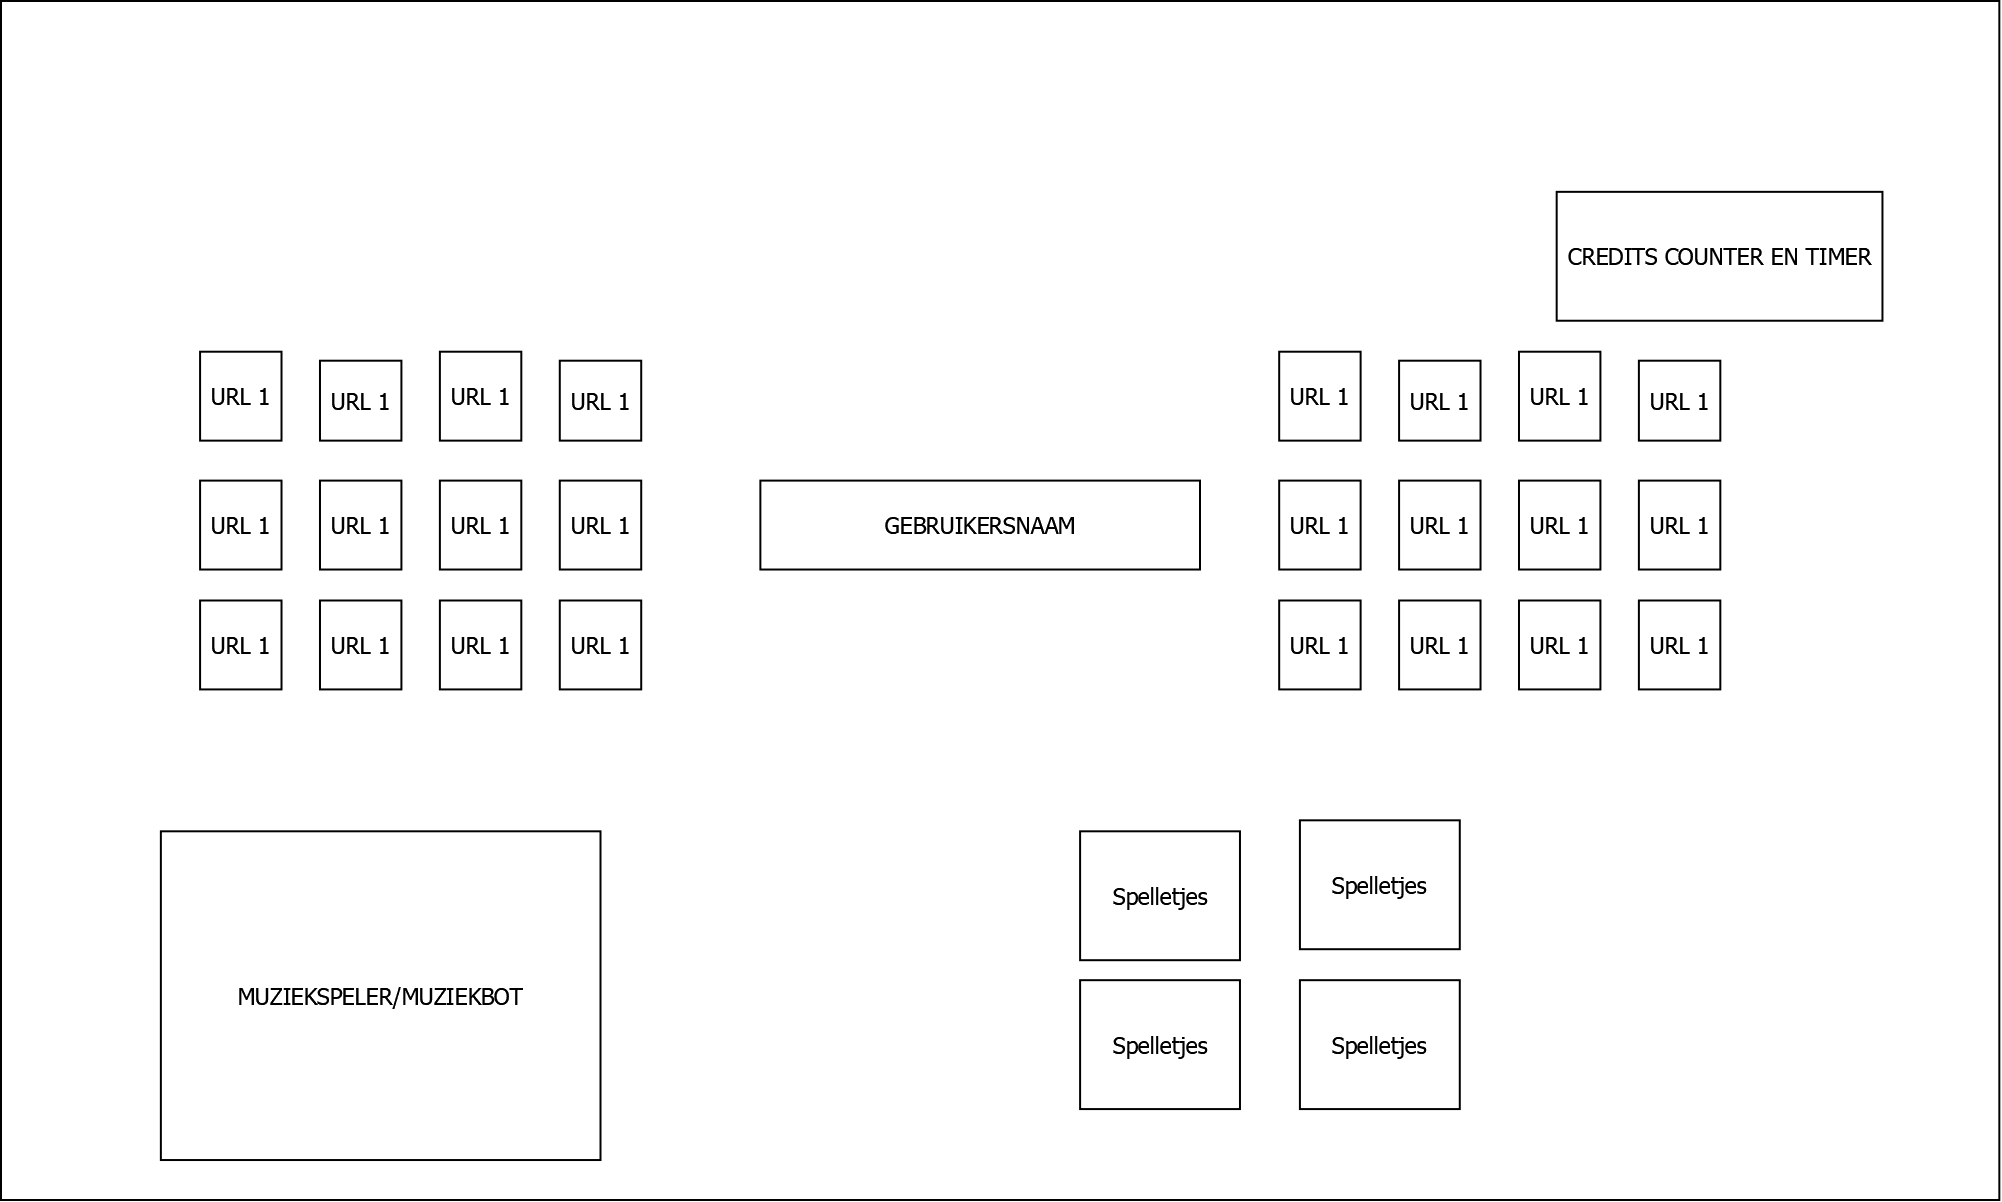
\includegraphics[width=\textwidth]{GUI}	
\end{figure}\\
\textbf{Niels: Zijn er nog meer deadlines nodig op deelproducten?\\
Timo: een duidelijk onderzoeksverslag skelet en VS project skelet.\\}
\newpage
	\item WVTTK (wat verder ten tafel komt)\\
		\textbf{Niels: Nee\\
		Tycho: Nope\\
		Timo: Niks}
	\item afsluiten\\
	\textbf{12:45 is de vergadering gesloten}\\
	
\end{itemize}

\paragraph{Nieuwe Actielijst}
\begin{itemize}
	\item Onderzoeksverslag (NIELS)
	\item bronverwijzing \LaTeX (TIMO)
	\item ERD databases 12-12-17 (TIMO)
	\item Indeling (CSS?) (TYCHO)
	\item beveiliging, login enzo... 
	\item Communiceren met server? (NIELS)
	\item Tegeltjes indeling/schalen? (TYCHO)
	\item Communicatie en besturing DaHause (TYCHO)
	\item Muziekbot/Muziekspeler (NIELS)
	\item Creditcounter + unlocken spelletjes (TIMO)
\end{itemize}

















\end{document}